% Chapter 6

\chapter{Results and Discussion} % Main chapter title

\label{Chapter6} % For referencing the chapter elsewhere, use \ref{Chapter6} 

\lhead{Chapter 6. \emph{Results and Discussion}} % This is for the header on each page - perhaps a shortened title

%----------------------------------------------------------------------------------------

\section{Introduction}
In chapter 5, Software Design Description (SDD) was explained. System architecture, main components and their functionalities, as well as components interaction were discussed. In this chapter, experiments of different classification procedures, dataset splits and feature selection are presented. Results are introduced in section 6.3. The discussion and analysis of obtained results are presented in section 6.4.


\section{Experimental Setup}

\subsection{Enron Dataset \cite{ENRON}}
Enron dataset is the most popular email corpus for research. It was released during the legal investigation into the Enron corporation.
it is an invaluable dataset since it contains uncensored messages from a corporate environment. The dataset consists of employee’s email folders, so it is also an accurate depiction of how users use folders. The majority of email directories in the dataset are small. So seven users with the largest email directories are chosen. Those seven users are chosen in many related papers (e.g. Huang, Bekkerman and McCallum, 2004\cite{RON04}). \\Statistics of the seven users are shown in table \ref{enronStatsTable}:

\begin{center}
	\centering
	\begin{table}
		\begin{tabular}{ |  >{\centering} l |  >{\centering} p{1.75cm} |  >{\centering} p{1.75cm} |  >{\centering}p{1.75cm} |  >{\centering} p{1.75cm} |  >{\centering} p{1.75cm} | p{1.75cm} <{\centering} | }
		\hline

		User & Number \newline of \newline folders & Number \newline of \newline messages & Size of \newline smallest \newline folder \newline (messages) & Size of \newline largest \newline folder \newline (messages) & Size of \newline smallest \newline message \newline (words) & Size of \newline largest \newline message \newline (words) \\ \hline \hline

		Beck-s & 101 & 1971 & 3 & 166 & 45 & 2620 \\ \hline
		Farmer-d & 25 & 3672 & 5 & 1192 & 43 & 3507 \\ \hline
		Kamniski-v & 41 & 4477 & 3 & 547 & 44 & 7885 \\ \hline
		Kitchen-l & 47 & 4015 & 5 & 715 & 47 & 46296 \\ \hline
		Lokay\_m & 11 & 2489 & 6 & 1159 & 45 & 4456 \\ \hline
		Sanders\_r & 30 & 1188 & 4 & 420 & 55 & 19331 \\ \hline
		Williams-w3 & 18 & 2769 & 3 & 1398 & 49 & 2287 \\ \hline
		\hline

		\end{tabular}
	\caption{Statistics on Enron datasets after removing non-topical and small folders.}
	\label{enronStatsTable}
	\end{table}
\end{center}



\subsection{Experiments}
Two types of experiments are reported:

\begin{itemize}
\item Learning Curves (Timeline): A learning curve is done by calculating the accuracy of each training/test split and plotting the classification accuracy curve over the number of training messages in the splits. 

\item Feature Comparison: Different combinations of possible classification features are selected and the accuracy of each combination is plotted. Each combination is run using both Naive Bayes and SVM algorithms.
\end{itemize}

\subsection{Training/test Set Splits}
In practice, the dataset grows over time. So, a natural way of splitting the dataset would be based on time: train on earlier emails and test on later ones. A similar approach is employed in (Klimt and Yang, 2004)\cite{KY04}. 
The incremental time-based split is done by sorting the emails according to their time stamp, then the classifier is trained on the first N messages and tested against the following N messages, then it is trained on the first 2N messages and tested against the following N messages etc. until we cover the whole dataset. N was chosen to be 100 which is similar to experiments conducted in (Bekkerman, McCallum and Huang 2004)\cite{RON04}.

\section{Results}

\subsection{Learning Curves}
Results of the seven Enron users are presented below as the accuracy over the timeline of each user.

\begin{figure}[H]
    \begin{center}
    \subfigure[beck-s]{
        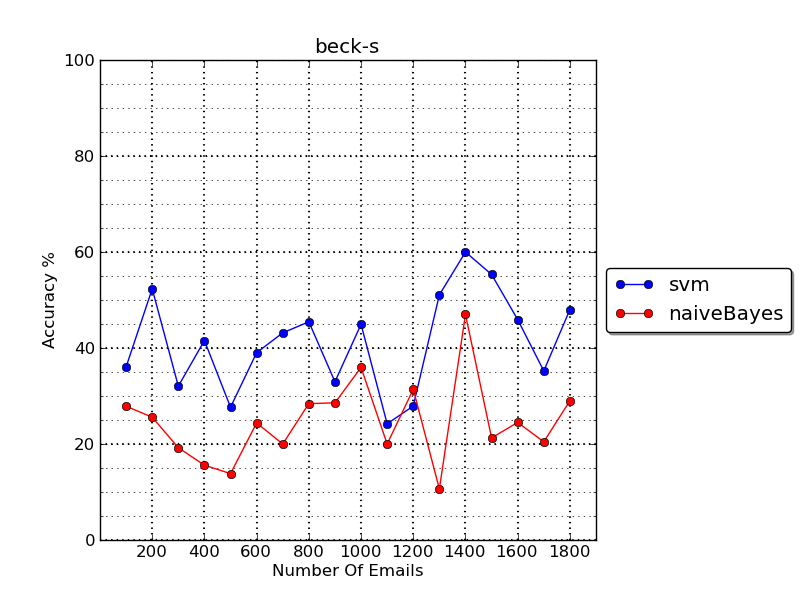
\includegraphics[scale=0.3]{beck-s.png}
    }
    \subfigure[farmer-d]{
        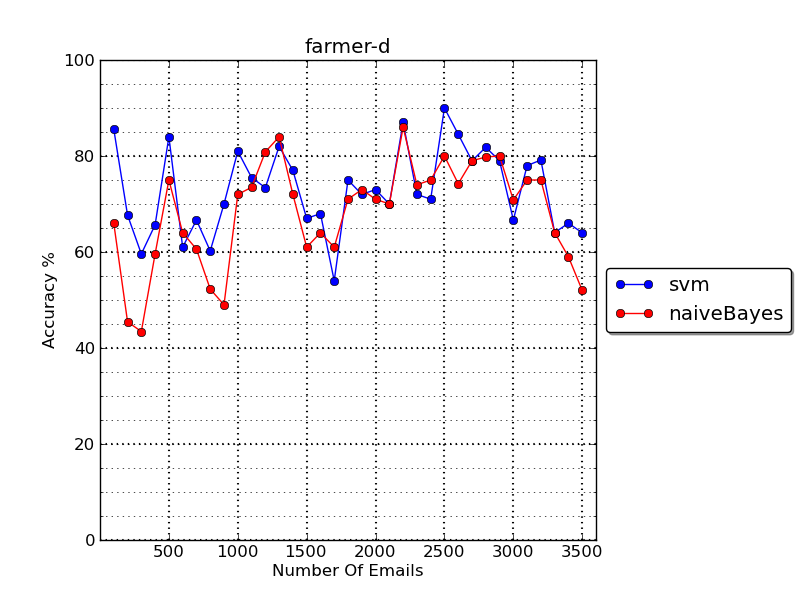
\includegraphics[scale=0.3]{farmer-d.png}
    }
    \subfigure[kamniski-v]{
        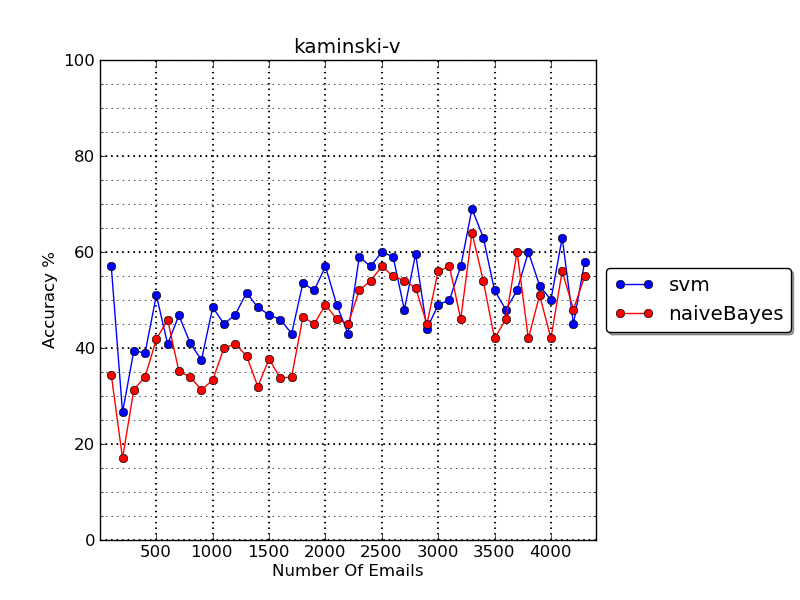
\includegraphics[scale=0.3]{kaminski-v.png}
    }
    \subfigure[kitchen-l]{
        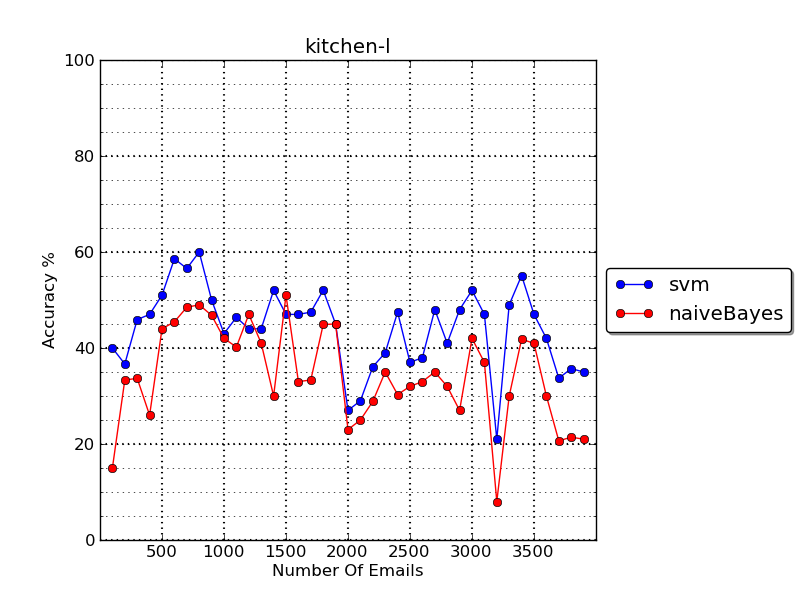
\includegraphics[scale=0.3]{kitchen-l.png}
    }
    \subfigure[lokay\_m]{
        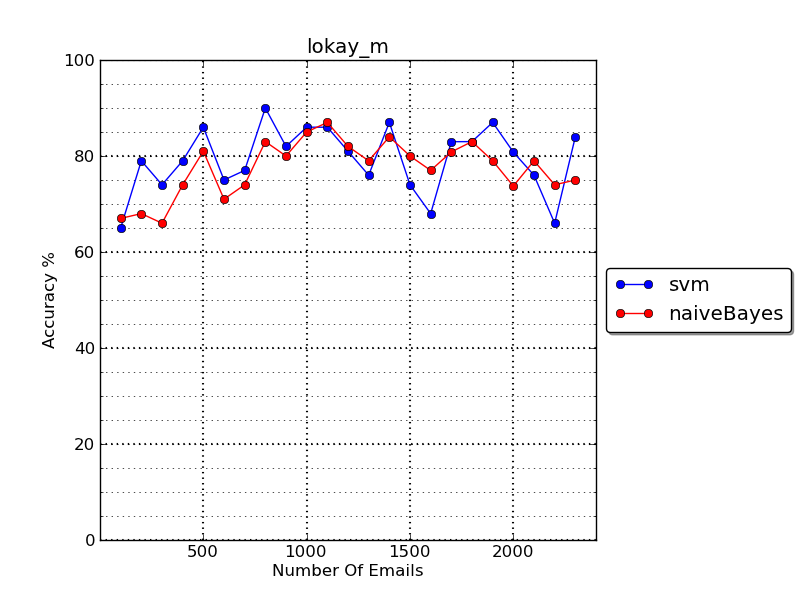
\includegraphics[scale=0.3]{lokay_m.png}
    }
    \subfigure[sanders\_r]{
        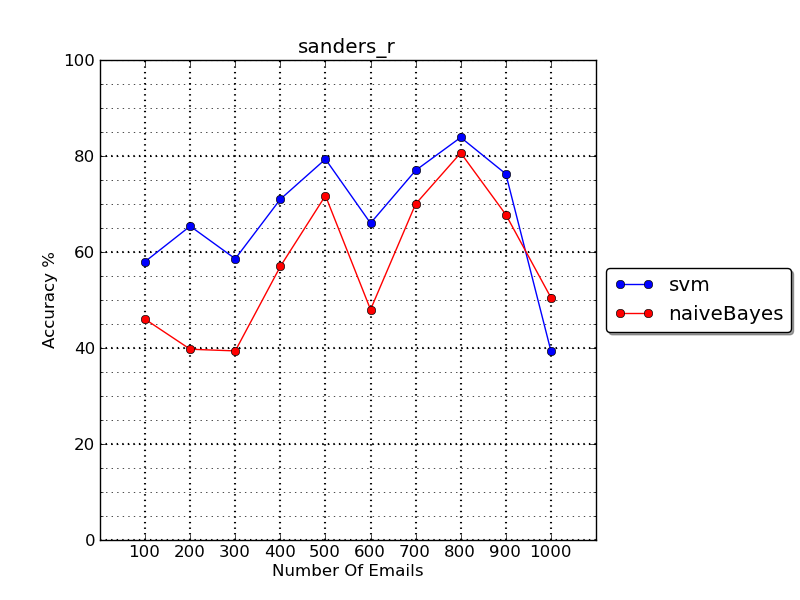
\includegraphics[scale=0.3]{sanders_r.png}
    }
    \subfigure[williams-w3]{
        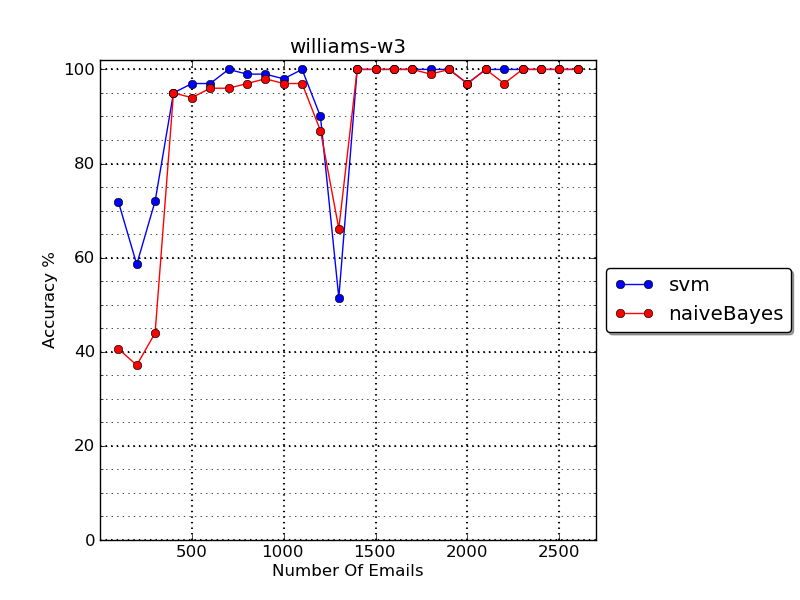
\includegraphics[scale=0.3]{williams-w3.png}
    }
    \end{center}
    \caption{Timeline results (learning curvers)}
\end{figure}

The following table is the accuracies averaged over all training/test splits for all users. It has two columns representing the 2 different classification algorithms: Naive Bayes and SVM.

\begin{table}
	\begin{center}

	    \begin{tabular}{ | l | l | l |}
	    \hline
	    User {\textbackslash}  Classifier & Naive Bayes & SVM \\ \hline
	    Beck-s & 24.65\% & 41.27\% \\ \hline
	    Farmer-d & 68.36\% & 72.87\% \\ \hline
	    Kamniski-v & 44.53\% & 50.36\% \\ \hline
	    Kitchen-l & 34.44\% & 44.15\% \\ \hline
	    Lokay\_m & 77.50\% & 79.34\% \\ \hline
	    Sanders\_r & 57.08\% & 67.49\% \\ \hline
	    Williams-w3 & 89.92\% & 93.30\% \\
	    \hline
	    \end{tabular}
	\caption{Average accuracy over all training/test splits}
	\end{center}
\end{table}

\subsection{Feature Comparison}
In classification, different combinations of the features affect accuracy. It is not necessarily that adding a feature will improve accuracy. So, it was important to test different features combinations to select the best combination. The results for six different combinations are reported below for each user. Each combination is tested under both Naive Bayes and SVM classification algorithms.

\begin{figure}[H]
    \begin{center}
    \subfigure[beck-s]{
        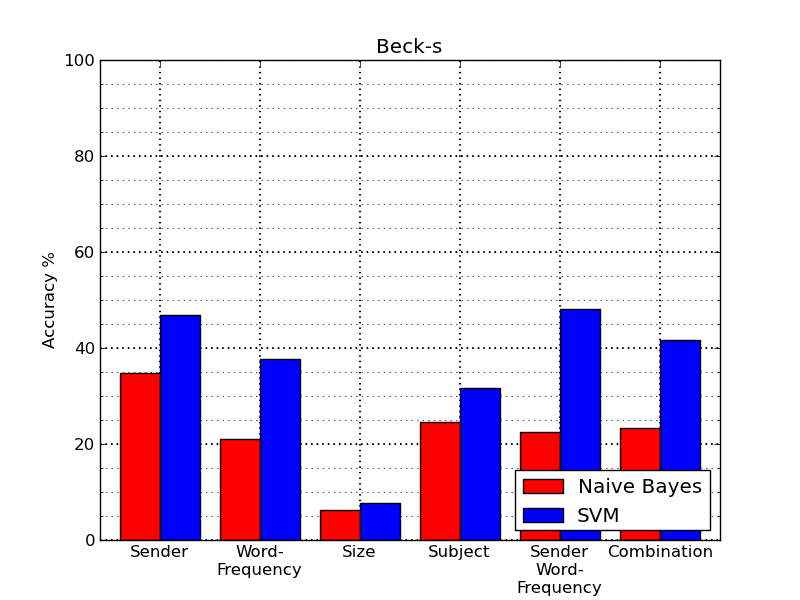
\includegraphics[scale=0.3]{F_Beck-s.png}
    }
    \subfigure[farmer-d]{
        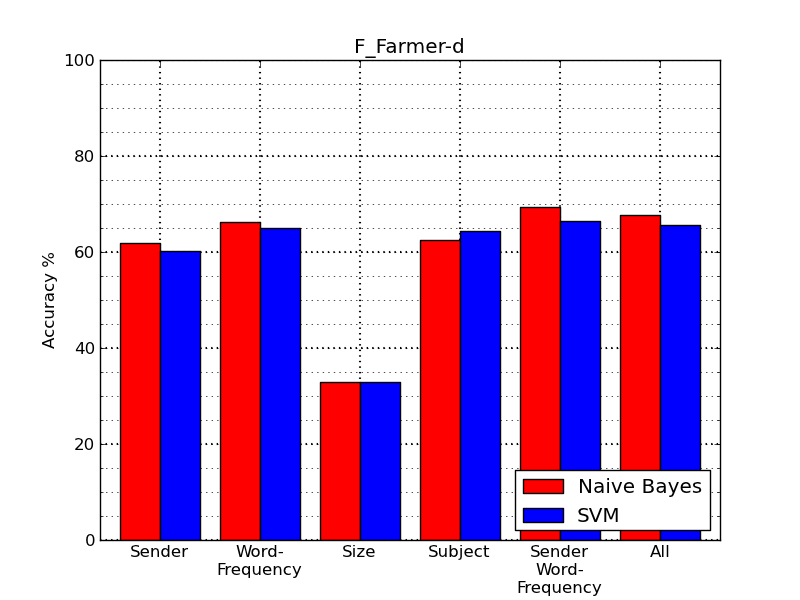
\includegraphics[scale=0.3]{F_Farmer-d.png}
    }
    \subfigure[kamniski-v]{
        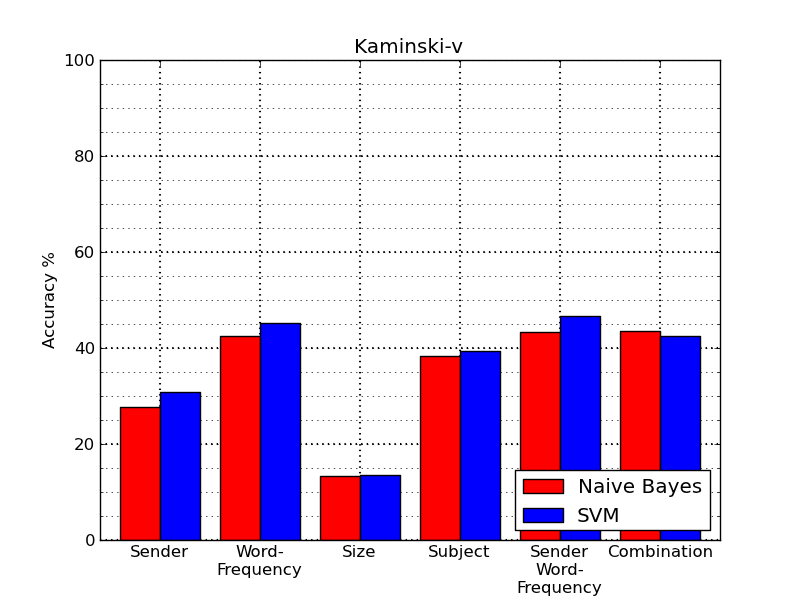
\includegraphics[scale=0.3]{F_Kaminski-v.png}
    }
    \subfigure[kitchen-l]{
        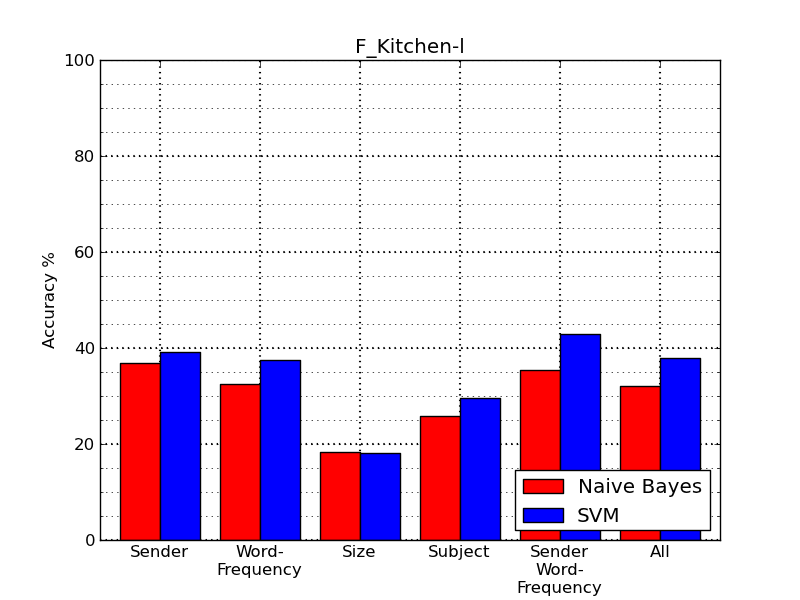
\includegraphics[scale=0.3]{F_Kitchen-l.png}
    }
    \subfigure[lokay\_m]{
        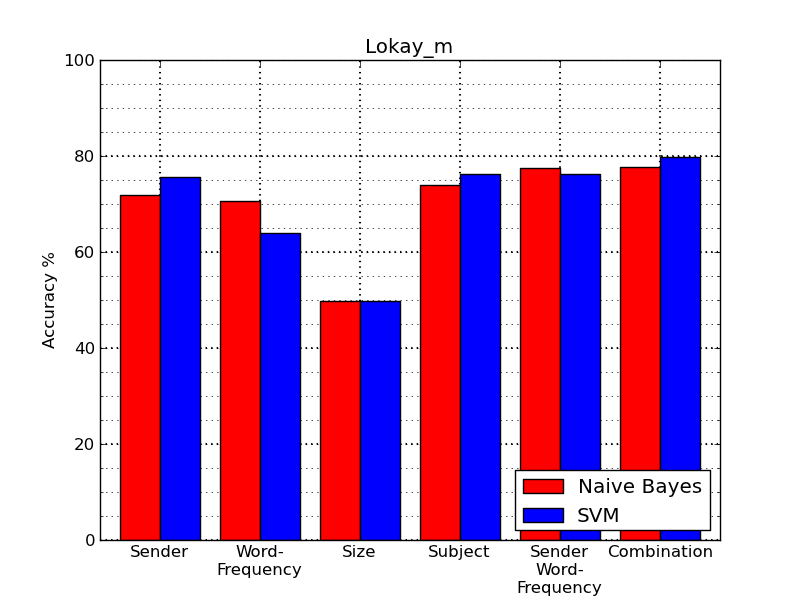
\includegraphics[scale=0.3]{F_Lokay_m.png}
    }
    \subfigure[sanders\_r]{
        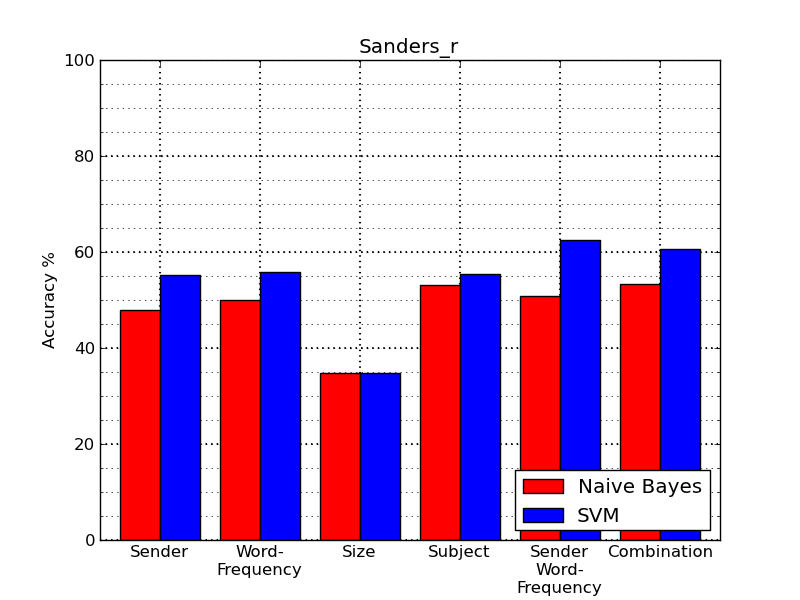
\includegraphics[scale=0.3]{F_Sanders_r.png}
    }
    \subfigure[williams-w3]{
        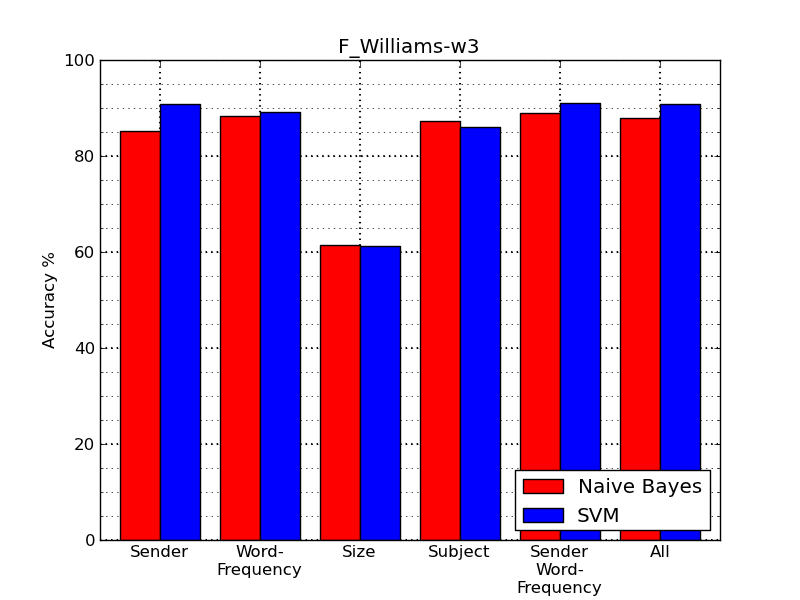
\includegraphics[scale=0.3]{F_Williams-w3.png}
    }
    \end{center}
    \caption{Results of different features combinations}
\end{figure}

\section{Discussion}
Learning curves show that SVM outperforms Naive Bayes in most of the cases. This is the expected behaviour. It is widely believed that Naive Bayes is not the best algorithm for text categorization (Dumais et al., 1998)\cite{DHS98}.
However, the results obtained doesn't reveal significance superiority of SVM over Naive Bayes. In fact, in some cases Naive Bayes was better than SVM (e.g Farmer-d feature selection figure). This is probably due to features selection and how the classifier weights each feature.


Experimental results obtained support the following observations:
\begin{itemize}
\item Accuracies are higher when the dataset has one or two dominant folders. As it can be seen from Table \ref{enronStatsTable}
 the size of the largest folder is nearly one half size of the entire dataset (e.g., users lokay\_m and williams-w3).

\item Newly created folders negatively affects the classification accuracy. If a new folder is created, the classifier trains on few emails from this folder which may not be enough to build a good classification model. (e.g see the drops in sanders\_r and william-w3 learning curves)

\item The dataset of user williams-w3 is a degenerative case. It has two large folders ("bill williams iii" and "schedule crawler" which contain most of the messages. This explains the high accuracy for this dataset regardless of the features used.

%TODO add more points (about feature comparison)
\end{itemize}

\section{Conclusion}
In this chapter the experimental results were presented. Analysis of the results were discussed. The results reveal the difficulty of eamil classification. Improving the accuracy is listed as a future work.

